\chapter{Introducci\'on}
\label{cap:intro}
En este capítulo el lector encontrará los elementos y conceptos introductorios necesarios para el entendimiento de este trabajo de título. 

\section{Antecedentes y motivaci\'on}
\label{intro:motivacion}

Con el paso del tiempo la tecnología avanza de forma considerable, lo que ha permitido el desarrollo de distintas áreas de la ciencia. Una de ellas es la Biología, área capaz de generar grandes volúmenes de información. Todo este conjunto de datos debe ser evaluado y estudiado, es así como nace la Bioinformática, campo de la Informática centrada en apoyar a la biología mediante el análisis y procesamiento de información biológica (\citealp{bioinf:def}).

Dentro de la Bioinformática, se encuentra la Bioinformática Estructural que se encarga principalmente del análisis y predicción de las estructuras tridimensionales de macro-moléculas biológicas (\citealp{bioinf:struct}), como el ADN, ARN y proteínas. El problema de la predicción de la estructura tridimensional de la proteína se conoce por sus siglas en inglés como \textit{3-D PSP (Three-dimensional Protein Structure Prediction) Problem} y es en el cual se basa este trabajo.

La estructura 3-D de la proteína da importante información acerca de su función biológica. Por ejemplo, la hemoglobina es la proteína encargada de transportar oxígeno en la sangre, para ello debe poseer una estructura tridimensional adecuada para poder realizar dicha tarea, para ello debe poseer zonas de anclaje que permitan a la hemoglobina captar moléculas de oxígeno. Por lo tanto, si se logra simular la estructura de tridimensional con una precisión alta implicaría un paso importante en el diseño de proteínas con fines específicos, lo anterior corresponde a la base del desarrollo de fármacos y drogas (\citealp{Cohen19961}).

No obstante, a pesar de los avances científicos, este problema sigue siendo costoso computacionalmente debido a la gran cantidad de recursos que se necesita para la simulación de interacciones moleculares. Además estas simulaciones se efectúan bajo la siguiente restricción biológica: la formación de la estructura tridimensional de la proteína se debe realizar usando la menor energía posible (\citealp{Anfinsen:1972}). Esto implica que cada modificación a nivel estructural tendrá repercución en la energía potencial libre del sistema, lo que complica y encarece el problema a nivel computacional.

Según lo revisado en \citealp{Zhang:2008}, se considera que los resultados cuyo RMSD entre $3-5\AA$ poseen una correcta topología, no asi aquellas que obtienen RMSD mayor a $9\AA$, de las cuales se dice que su topología es incorrecta. Además, menciona algunas técnicas que logran buenos resultados como ROSSETA (\citealp{Simons1997209}, con un promedio RMSD de $1.8\AA$ para la proteína CASP T0283 con 92 residuos de aminoácidos y un tiempo de 150 días de cómputo. I-TASSER (\citealp{PROT:PROT21702}) con resultados entre los $3-9\AA$ para proteínas de hasta 155 residuos y ASTRO-FOLD (\citealp{PROT:PROT20338}) con $5.2\AA$ para proteínas de 102 residuos.

\section{Descripci\'on del problema}
\label{intro:problema}

El problema de predicción de la estructura tridimensional de la proteína se resume en, encontrar la conformación tridimensional de la secuencia de aminoácidos con el mínimo de energía posible (\citealp{Anfinsen:1972}). Este problema pertenece al grupo NP-Completo (\citealp{Crescenzi:1998}) y se enmarca como uno de los principales desafíos en el área de la bioinformática estructural.

Las proteínas están compuestas por áminoácidos unidos mediantes enlaces. En estos enlaces se encuentran los ángulos de torsión o ángulos diedros que le dan la forma tridimensional a la proteína. El proceso de plegado ocurre de tal forma que la energía usada en este evento sea la mínima. Como se puede inferir, a medida que se aumenta la cantidad de residuos aumenta el espacio de soluciones debido a la cantidad de combinaciones posibles (\citealp{Zhang:2008}).

Los enlaces entre aminoácidos se conocen como enlaces peptídicos. Estos son producto de la interacción entre el grupo carboxilo y amino de los residuos. La principal particularidad que presentan las zonas enlazadas es la flexibilidad, que da origen a ángulos que terminan por dar forma al péptido. Estos ángulos son conocidos como diedros o de torsión, representados por las letras griegas $\phi$ y $\psi$ (\citealp{molecular:book}). Estos ángulos pueden tomar valores entre los $-180^{\circ}$ y $180^{\circ}$, es decir, para el par ($\phi$,$\psi$) existen $360{\times}360$ posibilidades, si la precisión de los ángulos se extiende a 3 decimales las posibilidades aumentan a $12.96{\times}10^{10}$. Por lo tanto, a medida que la proteína posee más residuos o aminoácidos, la cantidad de posibles conformaciones tridimensionales aumenta considerablemente lo que, en consecuencia, significa un espacio de búsqueda intratable. Desde el punto de vista de la dinámica molecular, es posible simular el proceso de plegado. No obstante, realizar esta simulación también es complicada y costosa computacionalmente hablando, debido a la gran cantidad de átomos, interacciones y variables termodinámicas involucradas. 

Para resolver este problema se han propuesto diversos enfoques, metodologías, sistemas y algoritmos que pueden ser agrupados en 4 clases:
\begin{itemize}
    \item Métodos \textit{ab initio} sin información de bases de datos.
    \item Métodos \textit{ab initio} con información de bases de datos.
    \item Métodos de enhebrado y reconocimiento de plegamientos.
    \item Métodos de modelamiento por comparación y estrategias de alineamiento de secuencias.
\end{itemize}
La primera clase corresponde a técnicas cuya principal ventaja es predecir estructuras nuevas o \textit{de novo} a través de la simulación de las propiedades físicoquímicas del proceso de plegamiento de la proteína. Las demás clases corresponden a métodos mucho más rápidos y efectivos para la predicción de estructuras tridimensionales, ya que hacen uso de plantillas estructurales y de bibliotecas de estructuras conformacionales conocidas (\citealp{Dorn2014251}). Estos enfoques serán explicados en detalle en la sección \ref{fundamentos:estado-arte} correspondiente al estado del arte.


\subsection{Enunciado del problema}
\label{intro:enunciado}
Dada una secuencia de aminoácidos se debe predecir la estructura tridimensional (estructura terciaria) de la proteína que representa.

\section{Soluci\'on propuesta}
\label{intro:solucion}

\subsection{Prop\'osito de la solución}

El propósito de la solución es, generar predicciones de proteínas a nivel de estructura terciaria usando los ángulos obtenidos de bases de datos experimentales. La idea de usar estos ángulos es disminuir el espacio de búsqueda, ya que se dejan de visitar aquellas regiones que los datos experimentales demuestran no tener relevancia. En la figura \ref{fig:rmc-proline} se puede apreciar que hay 2 zonas en las que se concentran los ángulos usados por el aminoácido \textit{Prolina}. Esto demuestra que no tiene sentido incluir en las simulaciones aquellas regiones que el aminoácido experimentalmente no usa. 

\begin{figure}[tp]
	\centering
	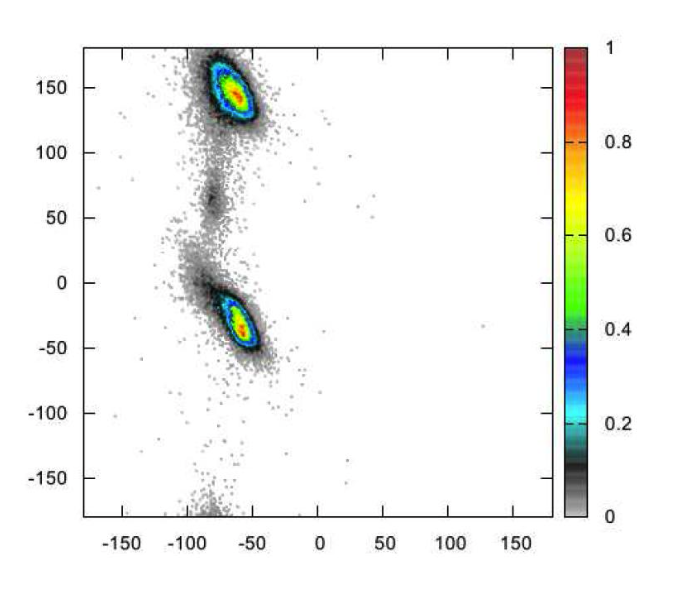
\includegraphics[scale=.35]{images/rmc-proline.png}
	\caption{\em Mapa de Ramachandran para las ocurrencias de los ángulos $\phi$ y $\psi$ encontrados en la Protein Data Bank para el amino\'acido Prolina (\citealp{Dorn:2013}).}
	\label{fig:rmc-proline} 
\end{figure}

Para llevar a cabo el propósito, se ha desarrollado un algoritmo memético que incorpora la información de los ángulos diedros más probables. Su objetivo es tomar y generar modelos candidatos de estructuras bajo la aplicación de operadores propios de los algoritmos evolutivos, que son mejorados mediante un operador de búsqueda local. El enfoque de esta solución está enmarcada dentro de las técnicas \textit{ab initio} que usan información de bases de datos cuya descripción detallada se encuentra en la sección \ref{fundamentos:abinitio-db}.

Los datos a emplear son provistos por la \textit{Protein Data Bank} (\citealp{Berman:2000}), que cuenta con la información de los ángulos de torsión $\phi$ y $\psi$ de estructuras conocidas y comprobadas experimentalmente a través de métodos de Cristalografía de Rayos X o Resonancia Magnética Nuclear (\textit{Nuclear Magnetic Resonance, NMR}). Para más detalle de estos métodos experimentales, revisar sección \ref{fundamentos:estructura-terciaria}.

\subsection{Alcances y limitaciones de la solución}

La solución enmarca las siguientes aristas y limitantes:

\begin{enumerate}[a)]
\item La solución propuesta contempla la evaluación e implementación solo para estructuras terciarias de proteínas y está basada en la solución propuesta en \cite{Dorn:2013}.
\item Solo se usan proteínas de acceso público disponibles en la \textit{Protein Data Bank} con solo una cadena principal de aminácidos.

\item Para el estudio y evaluación solo se consideran las proteínas 1DEP, 1E0Q, 1K43, 1L2Y, 1RPV y 2EVQ, cualquier otra proteína mencionada o evaluada en este trabajo es con fines ilustrativos.

\item No se considera una solución a nivel distribuido, por lo que la solución solo hace uso de los recursos provistos por el dispositivo de ejecución.
\end{enumerate}


\section{Objetivos}
\label{intro:objetivos}

En esta sección se dan a conocer los objetivos del presente trabajo, tanto en su enfoque general como en sus puntos específicos.

\subsection{Objetivo general}

El objetivo general de este trabajo es: la implementación de un algoritmo memético que incorpore conocimiento biológico y permita encontrar soluciones de buena calidad biológica para el problema \textit{3-D PSP}.

\subsection{Objetivos espec\'ificos}

Para la consecución del objetivo general, se plantean las siguientes metas intermedias:

\begin{enumerate}
  \item Reducción del espacio de búsqueda conformacional de la proteína, mediante el uso de una lista de probabilidades de ocurrencia (\textit{Angle Probability List, APL}) de pares de ángulos $\phi$ y $\psi$.
  \item Diseño e implementación del algoritmo memético que use la información biológica entregada por la APL.
  \item Diseño e implementación de un operador de búsqueda local para el algoritmo memético.
  \item Comparación y análsis de resultados con datos experimentales.
\end{enumerate}

\section{Metodolog\'ia y herramientas utilizadas}
\label{intro:metodologia}

\subsection{Metodolog\'ia}

Por tratarse de un tema de investigación y experimentación, se usará el método científico como metodología de foco para el desarrollo de este trabajo de título.

La hipótesis del trabajo es: \textbf{``Incorporar las probabilidades de ángulos de torsión $\phi$ y $\psi$ en un algoritmo memético permite obtener predicciones de estructuras tridimensionales de proteína de mejor calidad biológica''.}

No obstante, para realizar la etapa de experimentación para refutar o confirmar la hipótesis, es necesario la construcción de software, por lo que la metodología estará marcada por 4 etapas que se indican a continuación:

\begin{enumerate}
	\item \textbf{Concepción:} Se establecen los estudios necesarios para abordar el problema revisando alternativas y estrategias de solución.
	\item \textbf{Elaboración:} En esta etapa se definen modelos, esquemas y diagramas que se utilizan para construir la solución en base a la información recopilada en la concepción
	\item \textbf{Construcción:} Durante la construcción se implementan todos los elementos definidos durante la elaboración.
	\item \textbf{Experimentos computacionales y análsis de resultados:}: esta etapa recoge los resultados obtenidos a partir de la construcción para refinar y estabilizar el software. Se evalúa la hipótesis de acuerdo a los resultados obtenidos.
\end{enumerate}

\subsection{Herramientas de desarrollo}

A continuación se presentan las herramientas tanto de software como hardware que se utilizaron en este trabajo de título.

\subsubsection{Herramientas de software}
Para la escritura del documento se usaron las siguientes herramientas:
\begin{itemize}
	\item Sistema Operativo OS X Yosemite versión 10.10
	\item LaTeX para Mac, MacTex versión 2014
	\item TexStudio versión 2.8.8
\end{itemize}

Para el desarrollo, compilación y ejecución de las implementaciones se utilizó:

\begin{itemize}
	\item Sistema Operativo Linux Ubuntu Desktop versión 14.04.1 LTS
	\item Sublime Text versión 2.0.2
	\item AmberTools versión 14.23 (\citealp{amber14}).
	\item Stride (\citealp{Heinig01072004}).
	\item PyMol versión 1.6 (\citealp{pymol}).
	\item Procheck versión 3.5.4 (\citealp{procheck}).
	\item Profit versión 3.1 (\citealp{profit}).
\end{itemize}

\subsubsection{Herramientas de hardware}
Las ejecuciones de la implementación se llevaron a cabo en 10 computadores de escritorio modelo HP EliteDesk 800 G1-SFF con las siguientes características:

\begin{itemize}
	\item CPU Intel 3.4Ghz de 8 núcleos físicos.
	\item 8Gb de RAM (dos módulos de 8Gb de 1600Mhz).
\end{itemize}

\section{Organizaci\'on del documento}
\label{intro:organizacion}

El presente trabajo se compone por los siguientes capítulos:

\begin{itemize}
	%\item \textbf{Introducción: }este capítulo tiene la misión de introducir al lector en el contexto de este documento, abarcar los conceptos básicos para su entendimiento, enunciar el problema y solución propuesta, además de, mencionar la metodología y herramientas que usadas a lo largo del trabajo de titulación.
	\item \textbf{Capítulo 2. Fundamentos teóricos: }Para el entendimiento del problema es necesario definir y profundizar conceptos claves, que son usados en capítulos posteriores. Además se presenta el estado del arte de esta área.
	\item \textbf{Capítulo 3. Diseño e implementación de la solución: }este capítulo aborda el diseño de la solución propuesta en este trabajo. Por lo tanto, se menciona todo lo relacionado al algoritmo memético implementado, como la representación de las soluciones y el diseño algorítmico de los operadores.
	\item \textbf{Capítulo 4. Criterios de evaluación y experimentos: } Capítulo encargado de exponer la estrategia de evaluación y experimentación. En consecuencia, abarca el diseño de experimentos, carácterísticas y evaluación de las soluciones.
	\item \textbf{Capítulo 5. Resultados: }Los resultados de este trabajo están divididos en dos sub-secciones, la primera expone la calidad algorítmica de la implementación, tanto en la convergencia del algorítmo memético como en los parámetros que fueron usados en la etapa de experimentación.
La segunda evalúa los resultados a nivel biológico, se usan métricas que permiten evaluar la calidad biológica de los resultados obtenidos.
	\item \textbf{Capítulo 6. Conclusiones: }Finalmente se exponen las conclusiones obtenidas en este trabajo y se indican las posibles mejoras que puede tener para ser implementadas en un futuro.
\end{itemize}